% Topic from _Linear Algebra_ Jim Hefferon
%  http://joshua.smcvt.edu/linearalgebra
%  2012-Feb-12
\topic{Persegi Ajaib}
\index{persegi ajaib|(}
Sebuah legenda Tiongkok mengisahkan banjir di Sungai Lo.
Orang-orang mempersembahkan kurban untuk menenangkan sungai tersebut.
Setiap kali, seekor kura-kura muncul, berjalan mengelilingi persembahan, lalu
kembali ke air.
Fuh-Hi, % (2858-2738~BC)
pendiri peradaban Tiongkok, menafsirkan hal itu sebagai tanda bahwa sungai
masih murka. Untungnya, seorang anak memperhatikan bahwa tempurung kura-kura
tersebut memiliki pola di sebelah kiri bawah, yang kini disebut Lo Shu
(``gulungan sungai'').
\begin{center}
  \vcenteredhbox{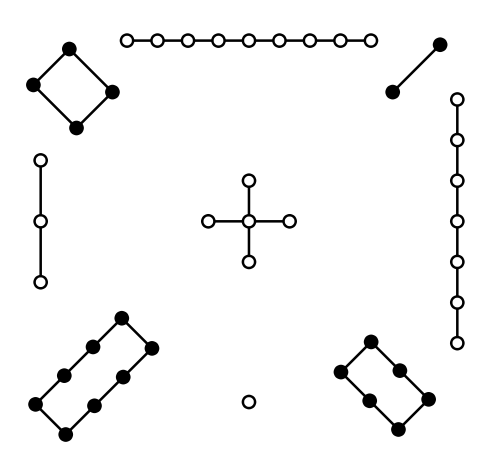
\includegraphics[height=.8in]{map/pix/LoShu.png}} % http://en.wikipedia.org/wiki/File:Lo_Shu_3x3_magic_square.svg
  \hspace{.8in}
  \begin{tabular}{|c|c|c|}
    \hline
      $4$  &$9$  &$2$  \\ \hline
      $3$  &$5$  &$7$  \\ \hline
      $8$  &$1$  &$6$  \\ \hline    
  \end{tabular}
\end{center}
Titik-titik itu membentuk matriks di sebelah kanan, yang setiap baris, kolom,
dan diagonalnya berjumlah $15$.
Setelah mengetahui seberapa banyak yang harus dipersembahkan, orang-orang
berhasil meredakan amarah sungai.
% (http://en.wikipedia.org/wiki/Lo_Shu_Square)

Matriks persegi disebut \definend{ajaib}\index{matriks!persegi ajaib}%
\index{persegi ajaib!definisi} jika setiap baris, kolom, dan diagonalnya
berjumlah sama, yaitu \definend{bilangan ajaib} matriks tersebut.

Persegi ajaib lain muncul dalam karya ukir \textit{Melencolia I} oleh D\"urer.
% (http://en.wikipedia.org/wiki/Melencolia_I)
\begin{center}
  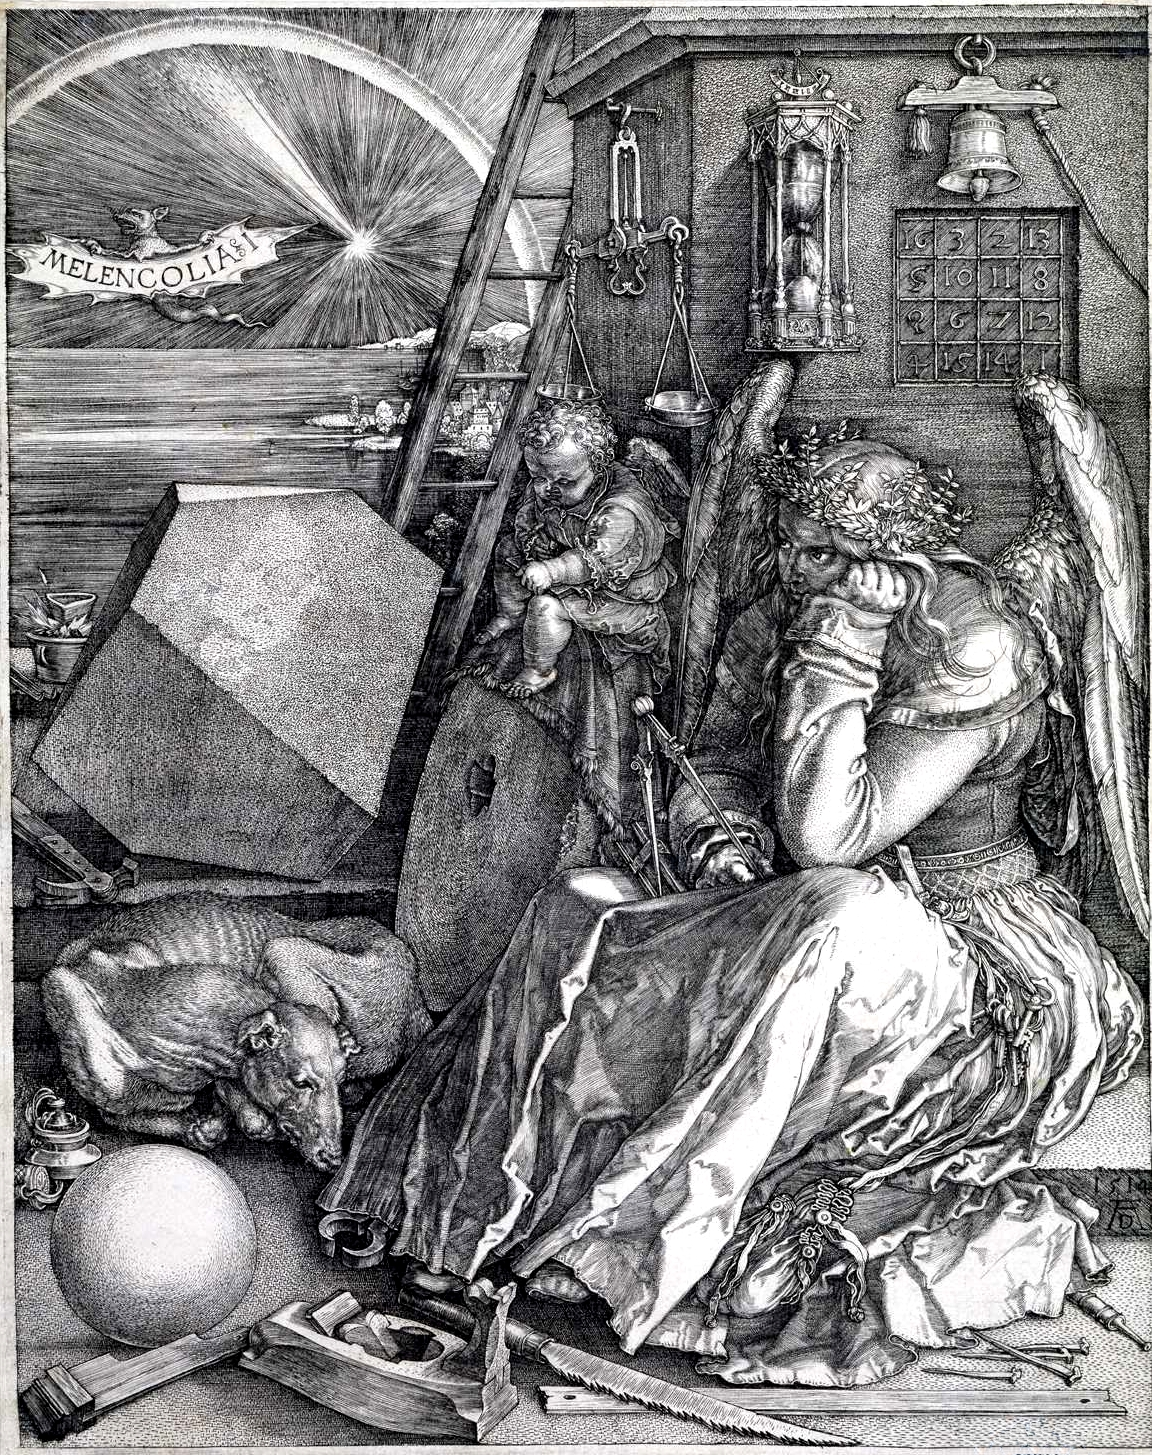
\includegraphics[height=2.20in]{map/pix/Melencolia.jpg} % wikipedia http://upload.wikimedia.org/wikipedia/commons/1/14/Melencolia_I_%28Durero%29.jpg
\end{center}
Salah satu penafsirannya adalah bahwa karya itu menggambarkan melankolia,
keadaan tertekan. Sosok genius di dalamnya dikelilingi banyak benda menarik
untuk dijelajahi, termasuk jangka, bangun geometris, timbangan, dan jam pasir.
Namun, sosok tersebut tidak tergerak; semua benda itu tergeletak tanpa dipakai.
Salah satu kemungkinan sumber kegembiraan di kanan atas adalah matriks
$\nbyn{4}$ yang setiap baris, kolom, dan diagonalnya berjumlah~$34$.
\begin{center}
  \vcenteredhbox{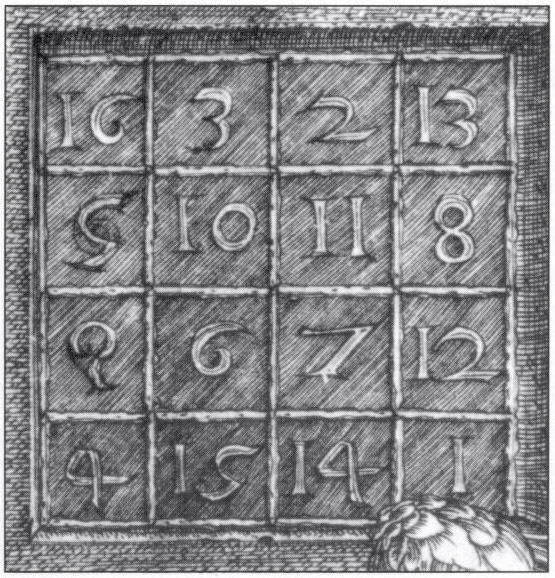
\includegraphics[height=1.25in]{map/pix/Melencoliadetail.jpg}} % wikipedia http://upload.wikimedia.org/wikipedia/commons/7/7e/Albrecht_D%C3%BCrer_-_Melencolia_I_%28detail%29.jpg
  \hspace{.8in}
  \begin{tabular}{|c|c|c|c|}
    \hline
      $16$  &$3$  &$2$  &$13$  \\ \hline
      $5$   &$10$ &$11$ &$8$   \\ \hline
      $9$   &$6$  &$7$  &$12$  \\ \hline    
      $4$   &$15$ &$14$ &$1$  \\ \hline  
  \end{tabular}
\end{center}
Dua entri tengah pada baris terbawah membentuk $1514$, tahun pembuatan karya
ukir tersebut.

Kedua persegi di atas merupakan susunan bilangan dalam
$\interval{1}{n^2}$. Keduanya disebut \definend{normal}%
\index{persegi ajaib!normal}.
Persegi $\nbyn{1}$ yang satu-satunya entrinya adalah $1$ bersifat normal;
\nearbyexercise{exer:TwoByTwoMagicSqUnique} menunjukkan bahwa tidak terdapat
persegi ajaib normal $\nbyn{2}$; dan terdapat persegi ajaib normal untuk setiap
ukuran lainnya; lihat \cite{WikipediaMagicSquare}.
Menentukan banyak persegi ajaib normal bagi setiap ukuran merupakan persoalan
yang belum terpecahkan; lihat \cite{OnlineEncyclopedia}.
 
Jika persegi-persegi itu tidak harus normal, kita dapat menyatakan jauh lebih
banyak. Setiap persegi $\nbyn{1}$ jelas bersifat ajaib.
Jika baris, kolom, dan diagonal matriks $\nbyn{2}$
\begin{equation*}
  \begin{mat}
    a  &b  \\
    c  &d
  \end{mat}
\end{equation*}
berjumlah~$s$, maka $a+b=s$, $c+d=s$, $a+c=s$, $b+d=s$, $a+d=s$, dan
$b+c=s$. \nearbyexercise{exer:TwoByTwoMagicSqUnique} menunjukkan bahwa sistem
ini memiliki solusi tunggal $a=b=c=d=s/2$.
Jadi, himpunan persegi ajaib $\nbyn{2}$ merupakan subruang berdimensi satu dari
$\matspace_{\nbyn{2}}$.

Jumlah dua persegi ajaib berukuran sama bersifat ajaib, dan kelipatan skalar
suatu persegi ajaib juga bersifat ajaib. Karena itu, himpunan persegi ajaib
$\nbyn{n}$, yaitu $\magicsquares_n$, merupakan ruang vektor, yakni subruang
dari $\matspace_{\nbyn{n}}$.
Topik ini menunjukkan bahwa untuk $n\geq 3$, dimensi $\magicsquares_n$ adalah
$n^2-2n$.
Himpunan $\magicsquares_{n,0}$ yang terdiri atas persegi ajaib $\nbyn{n}$
dengan bilangan ajaib~$0$ merupakan subruang lain. Kita juga akan memverifikasi
rumus dimensinya:~$n^2-2n-1$ ketika $n\geq 3$.

Pertama-tama, kita akan membuktikan bahwa
$\dim\magicsquares_n=\dim\magicsquares_{n,0}+1$.
Definisikan \definend{teras}\index{teras}\index{matriks!teras} suatu
matriks sebagai jumlah sepanjang diagonal dari kiri atas ke kanan bawah,
$\trace (M)=m_{1,1}+\cdots+m_{n,n}$.
Tinjau pembatasan teras pada persegi-persegi ajaib,
$\map{\trace}{\magicsquares_n}{\Re}$.
Ruang nol $\nullspace{\trace}$ merupakan himpunan persegi ajaib dengan bilangan
ajaib nol, yaitu $\magicsquares_{n,0}$.
Perhatikan bahwa teras bersifat surjektif karena untuk sebarang~$r$ dalam
kodomain $\Re$, matriks $\nbyn{n}$ yang semua entrinya $r/n$ merupakan persegi
ajaib dengan bilangan ajaib~$r$.
Teorema~Dua.II.\ref{th:RankPlusNullEqDim} menyatakan bahwa bagi sebarang
pemetaan linear, dimensi domain sama dengan dimensi ruang hasil ditambah
dimensi ruang nol, yaitu peringkat pemetaan ditambah nulitasnya.
Di sini domainnya adalah $\magicsquares_n$, ruang hasilnya $\Re$, dan ruang
nolnya $\magicsquares_{n,0}$, sehingga
$\dim\magicsquares_n=1+\dim\magicsquares_{n,0}$.

Kita akan menyelesaikannya dengan menemukan dimensi ruang vektor
$\magicsquares_{n,0}$.
Untuk $n=1$, dimensinya jelas $0$.
\nearbyexercise{exer:DimTwoMagicSqsMagicSumZero} menunjukkan bahwa
$\dim\magicsquares_{n,0}$ juga $0$ untuk $n=2$.

Yang tersisa adalah menunjukkan bahwa
$\dim\magicsquares_{n,0}=n^2-2n-1$ untuk $n\geq 3$.
Fakta bahwa persegi-persegi dalam ruang vektor ini bersifat ajaib memberikan
suatu sistem pembatas linear, dan fakta bahwa bilangan ajaibnya nol membuat
sistem tersebut homogen. Sebagai contoh, tinjau kasus $\nbyn{3}$.
Syarat bahwa baris, kolom, dan diagonal dari
\begin{equation*}
    \begin{mat}
      a &b &c \\
      d &e &f \\
      g &h &i
    \end{mat}
\end{equation*}
berjumlah nol memberikan sistem linear $\nbym{(2n+2)}{n^2}$ berikut.
\begin{equation*}
  \begin{linsys}{9}
    a &+ &b &+ &c &  &  &  &  &  &  &  &  &  &  &  &  &= &0 \\ 
      &  &  &  &  &  &d &+ &e &+ &f &  &  &  &  &  &  &= &0 \\ 
      &  &  &  &  &  &  &  &  &  &  &  &g &+ &h &+ &i &= &0 \\ 
    a &  &  &  &  &+ &d &  &  &  &  &+ &g &  &  &  &  &= &0 \\ 
      &  &b &  &  &  &  &+ &e &  &  &  &  &+ &h &  &  &= &0 \\ 
      &  &  &  &c &  &  &  &  &+ &f &  &  &  &  &+ &i &= &0 \\ 
    a &  &  &  &  &  &  &+ &e &  &  &  &  &  &  &+ &i &= &0 \\ 
      &  &  &  &c &  &  &+ &e &  &  &+ &g &  &  &  &  &= &0    
  \end{linsys}
\end{equation*}
Kita akan menemukan dimensi ruang tersebut dengan menentukan banyak variabel
bebas dalam sistem linear.

Matriks koefisien bagi kasus khusus $n=3$ dan~$n=4$ ditampilkan di bawah,
dengan baris dan kolom diberi nomor untuk membantu membaca pembuktian.
Terhadap basis standar, masing-masing merepresentasikan pemetaan linear
$\map{h}{\Re^{n^2}}{\Re^{2n+2}}$.
Domainnya berdimensi~$n^2$. Jadi, jika kita menunjukkan bahwa peringkat matriks
adalah $2n+1$, kita memperoleh hasil yang diinginkan, yakni dimensi ruang nol
$\magicsquares_{n,0}$ adalah $n^2-(2n+1)$.
\newlength{\interblockhspace}
\setlength{\interblockhspace}{1.45em}
\newlength{\interblockvspace}
\setlength{\interblockvspace}{1ex}
\newlength{\colwidth}
\settowidth{\colwidth}{$9$}
\begin{equation*}
  \begin{array}{r|ccc@{\hspace*{\interblockhspace}}ccc@{\hspace*{\interblockhspace}}ccc}
    \multicolumn{1}{c}{\ }  &1 &2 &3 &4 &5 &6 &7 &8 &9 \\
    \cline{2-10}
    \vec{\rho}_1 &1 &1 &1 &0 &0 &0 &0 &0 &0 \\
    \vec{\rho}_2 &0 &0 &0 &1 &1 &1 &0 &0 &0 \\
    \vec{\rho}_3 &0 &0 &0 &0 &0 &0 &1 &1 &1 \\[\interblockvspace]
    \vec{\rho}_4 &1 &0 &0 &1 &0 &0 &1 &0 &0 \\
    \vec{\rho}_5 &0 &1 &0 &0 &1 &0 &0 &1 &0 \\
    \vec{\rho}_6 &0 &0 &1 &0 &0 &1 &0 &0 &1 \\[\interblockvspace]
    \vec{\rho}_7 &1 &0 &0 &0 &1 &0 &0 &0 &1 \\
    \vec{\rho}_8 &0 &0 &1 &0 &1 &0 &1 &0 &0 
  \end{array}
\end{equation*}
\begin{equation*}
  \begin{array}{r|cccc@{\hspace*{\interblockhspace}}cccc@{\hspace*{\interblockhspace}}cccc@{\hspace*{\interblockhspace}}cccc}
    \multicolumn{1}{c}{\ }  &1 &2 &3 &4 &5 &6 &7 &8 &9 
           &\makebox[\colwidth]{$10$} &\makebox[\colwidth]{$11$} 
           &\makebox[\colwidth]{$12$} &\makebox[\colwidth]{$13$} 
           &\makebox[\colwidth]{$14$} &\makebox[\colwidth]{$15$} 
           &\makebox[\colwidth]{$16$} \\
    \cline{2-17}
    \vec{\rho}_1   &1 &1 &1 &1  &0 &0 &0 &0  &0 &0 &0 &0  &0 &0 &0 &0 \\
    \vec{\rho}_2   &0 &0 &0 &0  &1 &1 &1 &1  &0 &0 &0 &0  &0 &0 &0 &0 \\
    \vec{\rho}_3   &0 &0 &0 &0  &0 &0 &0 &0  &1 &1 &1 &1  &0 &0 &0 &0 \\
    \vec{\rho}_4   &0 &0 &0 &0  &0 &0 &0 &0  &0 &0 &0 &0  &1 &1 &1 &1 \\[\interblockvspace]
    \vec{\rho}_5   &1 &0 &0 &0  &1 &0 &0 &0  &1 &0 &0 &0  &1 &0 &0 &0 \\
    \vec{\rho}_6   &0 &1 &0 &0  &0 &1 &0 &0  &0 &1 &0 &0  &0 &1 &0 &0 \\
    \vec{\rho}_7   &0 &0 &1 &0  &0 &0 &1 &0  &0 &0 &1 &0  &0 &0 &1 &0 \\
    \vec{\rho}_8   &0 &0 &0 &1  &0 &0 &0 &1  &0 &0 &0 &1  &0 &0 &0 &1 \\[\interblockvspace]
    \vec{\rho}_9   &1 &0 &0 &0  &0 &1 &0 &0  &0 &0 &1 &0  &0 &0 &0 &1 \\
    \vec{\rho}_{10} &0 &0 &0 &1  &0 &0 &1 &0  &0 &1 &0 &0  &1 &0 &0 &0 \\
  \end{array}
\end{equation*}

Kita ingin menunjukkan bahwa peringkat matriks koefisien, yaitu banyak baris dalam
suatu himpunan bebas linear maksimal, adalah $2n+1$.
Jumlah $n$~baris pertama matriks koefisien sama dengan jumlah $n$~baris berikutnya,
yaitu vektor yang semua komponennya satu.
Jadi, himpunan bebas linear maksimal harus menghilangkan sekurang-kurangnya
satu baris. Kita akan menunjukkan bahwa himpunan semua baris kecuali baris
pertama, $\setinterval{\vec{\rho}_2}{\vec{\rho}_{2n+2}}$, bebas linear.
Karena itu, tinjau relasi linear berikut.
\begin{equation*}
  c_2\vec{\rho}_2+\cdots+c_{2n}\vec{\rho}_{2n}
     +c_{2n+1}\vec{\rho}_{2n+1}+c_{2n+2}\vec{\rho}_{2n+2}=\zero
   \tag{$*$}
\end{equation*}

Sekarang perinciannya menjadi rumit.
Fokuslah pada bagian kiri bawah tabel.
Perhatikan bahwa, pada dua baris terakhir dan $n$ kolom pertama, terdapat satu
subbaris yang semua entrinya nol kecuali entri awal bernilai satu pada kolom~$1$
dan satu subbaris yang semua entrinya nol kecuali entri akhir bernilai satu
pada kolom~$n$.

Pertama, setelah $\vec{\rho}_1$ dihilangkan, kolom~$1$ dan kolom~$n$
masing-masing hanya memuat dua entri satu.
Karena satu-satunya baris dalam~($*$) dengan entri kolom~$1$ tak nol adalah
$\vec{\rho}_{n+1}$ dan $\vec{\rho}_{2n+1}$, yang entrinya sama-sama satu, kita
harus memiliki $c_{2n+1}=-c_{n+1}$.
Demikian pula, peninjauan entri ke-$n$ dari vektor-vektor dalam~($*$)
memberikan $c_{2n+2}=-c_{2n}$.

Selanjutnya, tinjau kolom-kolom di antara keduanya\Dash dalam tabel $n=3$,
ini hanya mencakup kolom~$2$, sedangkan dalam tabel $n=4$ mencakup kolom~$2$
dan~$3$. Setiap kolom semacam itu hanya memiliki satu entri satu.
Artinya, untuk setiap indeks kolom $j\in\setinterval{2}{n-1}$, kolom tersebut
hanya berisi nol kecuali satu entri bernilai satu pada baris~$n+j$, sehingga
$c_{n+j}=0$.

Lanjutkan ke blok kolom berikutnya, dari $n+1$ hingga~$2n$.
Kolom~$n+1$ hanya memiliki dua entri satu (karena $n\geq 3$, entri-entri satu
pada dua baris terakhir tidak terletak pada kolom pertama blok ini).
Jadi, $c_2=-c_{n+1}$ dan karena itu $c_2=c_{2n+1}$.
Demikian pula, dari kolom~$2n$ kita menyimpulkan bahwa $c_2=-c_{2n}$,
sehingga $c_2=c_{2n+2}$.

Karena $n\geq 3$, terdapat sekurang-kurangnya satu kolom dari kolom~$n+2$
hingga kolom~$2n-1$.
Pada sekurang-kurangnya satu kolom tersebut, entri satu muncul dalam
$\vec{\rho}_{2n+1}$.
Jika entri satu juga muncul pada kolom tersebut dalam $\vec{\rho}_{2n+2}$,
maka kita memiliki $c_2=-(c_{2n+1}+c_{2n+2})$, karena $c_{n+j}=0$ untuk
$j\in\setinterval{2}{n-1}$.
Jika entri satu tidak muncul pada kolom tersebut dalam $\vec{\rho}_{2n+2}$,
maka $c_2=-c_{2n+1}$.
Dalam kedua kasus, $c_2=0$, sehingga $c_{2n+1}=c_{2n+2}=0$ dan
$c_{n+1}=c_{2n}=0$.

Jika blok $n$ kolom berikutnya bukan blok terakhir, dengan cara serupa kita
menyimpulkan dari kolom pertamanya bahwa $c_3=c_{n+1}=0$.

Lanjutkan proses ini hingga kita mencapai blok kolom terakhir, yang bernomor
$(n-1)n+1$ hingga~$n^2$.
Karena $c_{n+1}=\cdots=c_{2n}=0$, kolom~$n^2$ memberikan
$c_n=-c_{2n+1}=0$.

Dengan demikian, peringkat matriks adalah $2n+1$, seperti yang diperlukan.

\medskip
Sumber klasik tentang persegi ajaib normal adalah \cite{Ball}.
Pembahasan lebih lanjut mengenai persegi Lo Shu terdapat dalam
\cite{WikipediaLoShuSquare}. Pembuktian yang diberikan di sini berawal dari
\cite{Ward}.

\begin{exercises}
  \item Misalkan $M$ merupakan persegi ajaib $\nbyn{3}$ dengan bilangan
    ajaib~$s$.
    \begin{exparts}
      \partsitem Buktikan bahwa jumlah entri-entri $M$ adalah $3s$.
      \partsitem Buktikan bahwa $s=3\cdot m_{2,2}$.
      \partsitem Buktikan bahwa $m_{2,2}$ merupakan rata-rata entri-entri pada
        barisnya, kolomnya, dan setiap diagonal.
      \partsitem Buktikan bahwa $m_{2,2}$ merupakan median entri-entri $M$.
    \end{exparts}
    \begin{answer}
      \begin{exparts}
        \partsitem Jumlah entri-entri $M$ adalah jumlah dari jumlah ketiga
          barisnya.
        \partsitem Pembatas pada entri-entri $M$ yang melibatkan entri tengah
          menghasilkan sistem berikut.
          \begin{equation*}
            \begin{linsys}{3}
              m_{2,1}  &+  &m_{2,2}  &+  &m_{2,3}  &=  &s  \\ 
              m_{1,2}  &+  &m_{2,2}  &+  &m_{3,2}  &=  &s  \\ 
              m_{1,1}  &+  &m_{2,2}  &+  &m_{3,3}  &=  &s  \\ 
              m_{1,3}  &+  &m_{2,2}  &+  &m_{3,1}  &=  &s  
            \end{linsys}
          \end{equation*}
          Menjumlahkan keempat persamaan tersebut menghitung setiap entri
          matriks tepat satu kali, kecuali entri tengah yang dihitung empat
          kali. Jadi, ruas kiri berjumlah $3s+3m_{2,2}$, sedangkan ruas kanan
          berjumlah $4s$. Karena itu, $3m_{2,2}=s$.
        \partsitem
          Baris kedua berjumlah $s$, sehingga
          $m_{2,1}+m_{2,2}+m_{2,3}=3m_{2,2}$, yang memberikan
          $(1/2)\cdot(m_{2,1}+m_{2,3})=m_{2,2}$.
          Hal yang sama berlaku bagi kolom dan diagonal-diagonalnya.
        \partsitem
          Menurut butir sebelumnya, $m_{2,1}$ dan $m_{2,3}$ keduanya sama
          dengan $m_{2,2}$, atau salah satunya lebih besar dan yang lain lebih
          kecil. Jadi, $m_{2,2}$ merupakan median himpunan
          $\set{m_{2,1},m_{2,2},m_{2,3}}$.
          Penalaran yang sama pada kolom kedua menunjukkan bahwa $m_{2,2}$
          merupakan median himpunan
          $\set{m_{1,2},m_{2,1},m_{2,2},m_{2,3},m_{3,2}}$.
          Memperluasnya ke kedua diagonal menunjukkan bahwa $m_{2,2}$ merupakan
          median himpunan semua entri.
      \end{exparts}
    \end{answer}
  \item \label{exer:TwoByTwoMagicSqUnique}
    Selesaikan sistem $a+b=s$, $c+d=s$, $a+c=s$, $b+d=s$, $a+d=s$, dan
    $b+c=s$.
    \begin{answer}
      Untuk sebarang $s$, kita memiliki
      \begin{multline*}
        \begin{amat}{4}
          1  &1  &0  &0  &s  \\
          0  &0  &1  &1  &s  \\
          1  &0  &1  &0  &s  \\
          0  &1  &0  &1  &s  \\
          1  &0  &0  &1  &s  \\
          0  &1  &1  &0  &s            
        \end{amat}
        \grstep[-\rho_1+\rho_5]{-\rho_1+\rho_3}
        \begin{amat}{4}
          1  &1  &0  &0  &s  \\
          0  &0  &1  &1  &s  \\
          0  &-1 &1  &0  &0  \\
          0  &1  &0  &1  &s  \\
          0  &-1 &0  &1  &0  \\
          0  &1  &1  &0  &s            
        \end{amat}                                            \\
        \grstep{\rho_2\leftrightarrow\rho_6}
        \begin{amat}{4}
          1  &1  &0  &0  &s  \\
          0  &1  &1  &0  &s  \\          
          0  &-1 &1  &0  &0  \\
          0  &1  &0  &1  &s  \\
          0  &-1 &0  &1  &0  \\
          0  &0  &1  &1  &s  
        \end{amat}
        \grstep[-\rho_2+\rho_4 \\ \rho_2+\rho_5]{\rho_2+\rho_3}
        \begin{amat}{4}
          1  &1  &0  &0  &s  \\
          0  &1  &1  &0  &s  \\          
          0  &0  &2  &0  &s  \\
          0  &0  &-1 &1  &0  \\
          0  &0  &1  &1  &s  \\
          0  &0  &1  &1  &s  
        \end{amat}
      \end{multline*}
      Solusi tunggalnya adalah $a=b=c=d=s/2$.
    \end{answer}
  \item \label{exer:DimTwoMagicSqsMagicSumZero} 
    Tunjukkan bahwa $\dim\magicsquares_{2,0}=0$.
    \begin{answer}
       Menurut latihan sebelumnya, satu-satunya anggotanya adalah
       $Z_{\nbyn{2}}$.
    \end{answer}
  \item   \label{exer:TraceIsLinear}
    Misalkan fungsi \definend{teras}
    $\trace (M)=m_{1,1}+\cdots+m_{n,n}$.
    Definisikan pula jumlah sepanjang diagonal lainnya,
    $\trace^* (M)=m_{1,n}+\cdots+m_{n,1}$.
    \begin{exparts}
      \partsitem 
        Tunjukkan bahwa kedua fungsi
        $\map{\trace,\trace^*}{\matspace_{\nbyn{n}}}{\Re}$
        bersifat linear.
      \partsitem
        Tunjukkan bahwa fungsi
       $\map{\theta}{\matspace_{\nbyn{n}}}{\Re^2}$
       yang diberikan oleh $\theta(M)=(\trace(M),\trace^*(M))$ bersifat linear.
     \partsitem
       Perumum butir sebelumnya.
    \end{exparts}
    \begin{answer}
      \begin{exparts}
        \partsitem
          Untuk $M,N\in\matspace_{\nbyn{n}}$, kita memiliki
          $\trace(cM+dN)=(cm_{1,1}+dn_{1,1})+\cdots+(cm_{n,n}+dn_{n,n})
          =(cm_{1,1}+\cdots+cm_{n,n})+(dn_{1,1}+\cdots+dn_{n,n})
          =c\cdot\trace(M)+d\cdot\trace(N)$, dengan semua bilangan bernilai
          riil, sehingga teras mempertahankan kombinasi linear.
          Argumen bagi $\trace^*$ serupa.
       \partsitem
         Fungsi tersebut mempertahankan kombinasi linear:~jika semua bilangan
         bernilai riil,
          $\theta(cM+dN)=(\trace(cM+dN),\trace^*(cM+dN))
          =(c\cdot\trace(M)+d\cdot\trace(N), c\cdot\trace^*(M)+d\cdot\trace^*(N))
          =c\cdot\theta(M)+d\cdot\theta(N)$.
       \partsitem   
         Jika $\map{h_1,\ldots,h_n}{V}{W}$ linear, maka pemetaan
         $\map{g}{V}{W^n}$ yang diberikan oleh
         $g(\vec{v})=(h_1(\vec{v}), \ldots, h_n(\vec{v}))$
         juga linear. Pembuktiannya mengikuti pembuktian butir sebelumnya.
      \end{exparts}
    \end{answer}
  \item Matriks persegi disebut \definend{semi-ajaib} jika baris dan kolomnya
     berjumlah sama; artinya, jika kita menghapus syarat pada diagonal.
     \begin{exparts*}
       \partsitem
         Tunjukkan bahwa himpunan persegi semi-ajaib $\semimagicsquares_n$
         merupakan subruang dari $\matspace_{\nbyn{n}}$.
       \partsitem
         Tunjukkan bahwa himpunan $\semimagicsquares_{n,0}$ yang terdiri atas
         persegi semi-ajaib $\nbyn{n}$ dengan bilangan ajaib~$0$ juga merupakan
         subruang dari $\matspace_{\nbyn{n}}$.
     \end{exparts*}
     \begin{answer}
       \begin{exparts*}
         \partsitem
           Jumlah dua persegi semi-ajaib bersifat semi-ajaib, demikian pula
           kelipatan skalar suatu persegi semi-ajaib.
         \partsitem
           Seperti pada butir sebelumnya, kombinasi linear dua persegi
           semi-ajaib dengan bilangan ajaib nol juga merupakan matriks semacam
           itu.
       \end{exparts*}
     \end{answer}
  % 2014-Dec-19 Nothing wrong with this; I trimmed to make pages fit.
  % \item 
  %   \cite{Beardon}
  %   Here is a slicker proof of the result of this Topic, when $n\geq 3$.
  %   See the prior two exercises for some definitions and needed results.
  %   \begin{exparts}
  %     \partsitem
  %       First show that 
  %       $\dim\magicsquares_{n,0}=\dim\semimagicsquares_{n,0}+2$.
  %       To do this, consider the function
  %       $\map{\theta}{\matspace_n}{\Re^2}$ sending a 
  %       matrix~$M$ to
  %       the ordered pair $(\trace(M),\trace^*(M))$.
  %       Specifically, consider the restriction of that map
  %       $\map{\theta}{\semimagicsquares_n}{\Re^2}$ to the semimagic squares.  
  %       Clearly its null space is $\magicsquares_{n,0}$.
  %       Show that when $n\geq 3$ this restriction $\theta$ is onto.
  %       (\textit{Hint:} we need only find a basis for 
  %          $\Re^2$ that is the
  %          image of two members of $\mathcal{H}_n$)  
  %     \partsitem
  %       Let the function $\map{\phi}{\matspace_{\nbyn{n}}}{\matspace_{\nbyn{(n-1)}}}$
  %       be the identity map except that it 
  %       drops the final row and column: $\phi(M)=\hat{M}$ where 
  %       $\hat{m}_{i,j}=m_{i,j}$ for all $i,j\in\setinterval{1}{n-1}$.
  %       The check that $\phi$ is linear is easy.
  %       Consider $\phi$'s restriction to the semimagic squares with 
  %       magic number zero
  %      $\map{\phi}{\semimagicsquares_{n,0}}{\matspace_{\nbyn{(n-1)}}}$.
  %      Show that $\phi$ is one-to-one
  %    \partsitem
  %      Show that $\phi$ is onto.
  %    \partsitem Conclude that
  %       $\semimagicsquares_{n,0}$ has dimension~$(n-1)^2$.
  %    \partsitem 
  %       Conclude that $\dim(\magicsquares_n)=n^2-n$
  %   \end{exparts}
  %   \begin{answer}
  %     \begin{exparts}
  %       \partsitem
  %         Consider the matrix $C\in \mathcal{H}_n$ that has all 
  %         entries zero except
  %         that the four corners are $c_{1,1}=c_{n,n}=1$ and $c_{1,n}=c_{n,1}=-1$.
  %          Also consider the matrix $D\in \mathcal{H}_n$ with all entries 
  %          zero except that 
  %          $d_{1,1}=d_{2,2}=1$ and $d_{1,2}=d_{2,1}=-1$.
  %          We have
  %          \begin{equation*}
  %             \theta(C)=\colvec{2 \\ -2}
  %             \qquad
  %             \theta(D)=\begin{cases}
  %                          \binom{2}{-1}  &\text{if $n=3$}  \\[1ex]
  %                          \binom{2}{0}  &\text{if $n>3$}
  %                       \end{cases}
  %          \end{equation*}
  %          and so the image of $\theta$ includes a basis for $\Re^2$ and
  %          thus $\theta$ is onto.
  %          With that, because for any linear map the
  %          dimension of the domain equals its rank plus its nullity
  %          we conclude that 
  %          $\dim(\mathcal{H}_n)=2+\dim(\magicsquares_{n,0})$, as desired.
  %       \partsitem
  %          We claim that 
  %          $\map{\phi}{\semimagicsquares_{n,0}}{\matspace_{\nbyn{(n-1)}}}$.
  %          is one-to-one and onto.

  %          To show that it is one-to-one we will show that the only member of 
  %          $\semimagicsquares_{n,0}$ mapped to the zero matrix $Z_{\nbyn{(n-1)}}$
  %          is the zero matrix~$Z_{\nbyn{n}}$.
  %          Suppose that $M\in\semimagicsquares_{\nbyn{n}}$ and 
  %          $\phi(M)=Z_{\nbyn{(n-1)}}$.
  %          On all but the final row and column $\phi$ is the identity so
  %          the entries in $M$ in all but the final row and column are zero: 
  %          $m_{i,j}=0$ for $i,j\in\setinterval{1}{n-1}$.
  %          The first row of $M$ adds to zero and hence
  %          the final entry in that row $m_{1,n}$ is zero.
  %          Similarly the final entry in each row $i\in\setinterval{1}{n-1}$
  %          and column $j\in\setinterval{1}{n-1}$ is zero.
  %          Then, the final column adds to zero so $m_{n,n}=0$.
  %          Therefore $M$ is the zero matrix $Z_{\nbyn{n}}$ and the 
  %          restriction of $\phi$ 
  %          is one-to-one. 
  %       \partsitem
  %          Consider a member $\hat{M}$ of the codomain $\matspace_{\nbyn{(n-1)}}$.
  %          We will produce a matrix $M$ from the domain 
  %          $\semimagicsquares_{n,0}$ that maps to it.
  %          The function $\phi$ is the identity on all but the final row 
  %          and column of 
  %          $M$ so for $i,j\in\setinterval{1}{n-1}$
  %          the entries are $m_{i,j}=\hat{m}_{i,j}$.
  %          \begin{equation*}
  %            M=\begin{mat}
  %              \hat{m}_{1,1}    &\hat{m}_{1,2}  &\ldots &\hat{m}_{1,n-1} &m_{1,n}  \\
  %              \vdotswithin{\hat{m}_{1,1}}  
  %                &\vdotswithin{\hat{m}_{1,2}}     \\
  %              \hat{m}_{n-1,1}  &\hat{m}_{n-1,2} &\ldots &\hat{m}_{n-1,n-1} &m_{n-1,n}  \\
  %              m_{n,1}         &m_{n,2}         &\ldots &m_{n,n-1}        &m_{n,n}  
  %           \end{mat}
  %         \end{equation*}
  %         The first row of $M$ must add to zero so we take $m_{1,n}$ to be  
  %         $-(\hat{m}_{1,1}+\cdots+\hat{m}_{1,n-1})$.
  %         In the same way we get the final entries 
  %         $m_{i,n}=-(\hat{m}_{i,1}+\cdots+\hat{m}_{i,n-1})$ in all the rows but the 
  %         bottom $i\in\setinterval{1}{n-1}$, 
  %         and the final entries $m_{n,j}=-(\hat{m}_{1,j}+\cdots+\hat{m}_{n-1,j})$ 
  %         in all the columns but the last
  %         $j\in\setinterval{1}{n-1}$.
  %         The entry remaining is the one in the lower right~$m_{n,n}$.
  %         The final column adds to zero so we set it to 
  %         $-(m_{1,n}+\cdots+m_{n-1,n})$ but we must check
  %         that the final row now also adds to zero.
  %         We have $m_{n,n}=-m_{1,n}-\cdots-m_{n-1,n}$ and expanding each of the
  %         $m_{i,n}$ as $-\hat{m}_{1,1}-\cdots-\hat{m}_{1,n-1}$
  %         gives that we have defined $m_{n,n}$ to be the sum of all the entries
  %         of $\hat{M}$.
  %         The sum of the all the entries but the last in the final row is
  %         $m_{1,n}+m_{2,n}+\cdots+m_{n-1,n}$ and expanding each 
  %         $m_{n,j}=-\hat{m}_{1,j}-\cdots-\hat{m}_{n-1,j}$ 
  %         verifies that the sum of the final row is zero.
  %         Thus $M$ is semimagic with magic number zero and so $\phi$ is onto.
  %       \partsitem
  %          Theorem~Two.II.\ref{th:RankPlusNullEqDim} says that for any linear 
  %          map the
  %          dimension of the domain equals its rank plus its nullity.
  %          Because $\map{\phi}{\semimagicsquares_n}{\matspace_{\nbyn{(n-1)}}}$ 
  %          is one-to-one its nullity is zero.
  %          Because it is onto its rank is $\dim(\matspace_{\nbyn{(n-1)}})=(n-1)^2$.
  %          Thus the domain of $\phi$, the subspace  
  %          $\semimagicsquares_{n,0}$ of semimagic squares with magic number zero,
  %          has dimension~$(n-1)^2$.
  %        \partsitem   
  %          We have that $\dim\magicsquares_n=\dim\magicsquares_{n,0}+1
  %          =(\dim\semimagicsquares_n-2)+1=(n-1)^2-1=n^2-n$ 
  %          when $n\geq 3$.
  %     \end{exparts}
  %   \end{answer}
\end{exercises}
\index{persegi ajaib|)}
\endinput
